\begin{task}{The Good Old Days}{1}
\In
An integer $4$.
\Out
The word \s{"Elephant"}.

\begin{ExampleIO}
\egio{4}{Elephant}
\end{ExampleIO}
\end{task}

\begin{task}{Echos In The Well}{1}
\In
String $S$ with no line breaks.
\Out
Said string $S$.

\begin{ExampleIO}
\egio{Hello}{Hello}
\end{ExampleIO}
\end{task}

\begin{task}{Equation of a Line}{1}
\In
Two integers $k$ and $b$, $k \neq 0$.
\Out
Such value $x$, that it satisfies the equation $kx+b=0$. 
\end{task}

\begin{task}{Wait, what?}{2}
\In
Two integers $a$ and $b$.
\Out
The product of $a$ and $b$.
\Note
You may not use the multiplication operation.

\begin{ExampleIO}
\egio{1\\0}{0}
\egio{7\\8}{56}
\end{ExampleIO}
\end{task}

\begin{task}{Late'o'clock}{2}
\In An integer $0 \leq h < 24$. Hours on a clock.
\Note Convert the given time $h$ to the 12-hour clock format.
\Out First the time $h$ in 12-hour clock format, then \s{"am"} or \s{"pm"}
depending on the time.

\begin{ExampleIO}
\egio{0}{12am}
\egio{8}{8am}
\egio{13}{1pm}
\end{ExampleIO}

\end{task}

\begin{task}{Quadratic Equations}{2}
\In
Three integers $a$, $b$ and $c$.
\Out
Find all values of $x$, such that $ax^2 + bx + c=0$. 
\Note
If there are no possible values of $x$ output \texttt{"NaN"} (not a number). 
The values should not be repeated.

\begin{ExampleIO}
\egio{1\\-1\\-6}{-2\\3}
\end{ExampleIO}

\end{task}

\begin{task}{Qubic Equation}{3}
\In
Four integers $a$, $b$, $c$ and $d$.
\Out
Find all values of $x$, such that $ax^3 + bx^2 + cx + d = 0$. 
\Note
If there are no possible values of $x$ output \texttt{"NaN"} (not a number). 
The values should not be repeated.
\Hint
use Cardano's formula.
\end{task}

\begin{task}{Euclid Approves}{1}
\In
Two integers $a$ and $b$, sides of a right angled triangle.
\Out
The hypotenuse $c$ of the aforementioned triangle.

\begin{ExampleIO}
\egio{3\\4}{5}
\end{ExampleIO}
\end{task}

\begin{task}{Euclid Disapproves}{2}
\In
Two integers $a$ and $b$, sides of a right angled triangle and an integer angle
$\theta$ (given in degrees) between them.
\Out
The third side of the triangle.
\Hint
You may use \s{import math} to get some functions you might want.
\end{task}

\begin{task}{Everyone but Euclid Approves}{3}
\In
An integer $n$ the amount of following lines, $3 \leq n \leq 100$. 
Each following line $i$ contains a number $-100 \leq a_i \leq 100$, a 
component of the vector $\hat{v} = \{a_1, a_2, \dots, a_n\}$.
\Out
The length of a vector $||\hat{v}||$.
\end{task}

\begin{task}{Minmaxed}{1}
\In
Two integers, $a$ and $b$.
\Out
Two integers, first the largest of them two, next the smallest.
\end{task}

\begin{task}{TreE}{3}
\In
An integer $h$, the height of the christmass tree.
\Out
A christmas tree with total height $h + 1$, $1$ being the trunk of said
tree and $h$ all the result of it.

\begin{ExampleIO}
\egio{4}{e\\
a a\\
e e e \\
a a a a\\
a}
\end{ExampleIO}
\end{task}

\begin{task}{Sigma for Sum}{2}
\In
An integer $a$ such that $1 \leq a \leq 10^{10^{10}}$.
\Out
The sum all the integers $1 + 2 + \dots + a$.
\Hint
Loop isn't the only way to go.
\end{task}

\begin{task}{Factor!al}{2}
\In
An integer $a$ such that $1 \leq b \leq 10^{5}$.
\Out
The product all the integers $1 \times 2 \times \cdots \times b$.
\Hint
Lookup the arguments for \s{range} in the official Python3.x documentation.
\end{task}

\begin{task}{Minmaxed 2: The Sequel}{3}
\In
Two integers, $a$ and $b$.
\Out
Two integers, first the largest of them two, next the smallest.
\Note
You may  only use \s{min()} or \s{max()}, not both. You may not use branching.
\end{task}

\begin{task}{Set Product}{2}
\In
Two integers, $a$ and $b$ where $a > 0$ and $b > 0$. They create sets of values:
$A = \{0, 1, \dots, a - 1\}$ and $B = \{0, 1, \dots, b - 1\}$.
\Out
Print out the product of the two sets.
\Note
A product of two sets is a mapping of every element of one set to every element
of another, e.g. for sets $C = \{1, 2\}$ and $D = \{3, 4\}$ the product is
$C \times D = \{(1, 3), (1, 4), (2, 3), (2, 4)\}$.
\end{task}

\begin{task}{Sheared Parallelogram}{5}
    A sheared parallelogram is drawn on a plane. The parallelogram has width $A$ and
    height $B$. All the sides of parallelogram are parallel to their respective
    opposing sides. Right and left sides are sheared by some angle $\alpha$.
    Corners of the sheared parallelogram are non-integers.
    \In
    Two non-negative real numbers $A$, $B$ and $\alpha$ (with 3
    decimal places at most), width, height and the angle in degrees respectively.
    \Out
    How many points with integer coordinates are enclosed inside the sheared
    parallelogram.

    \centering
    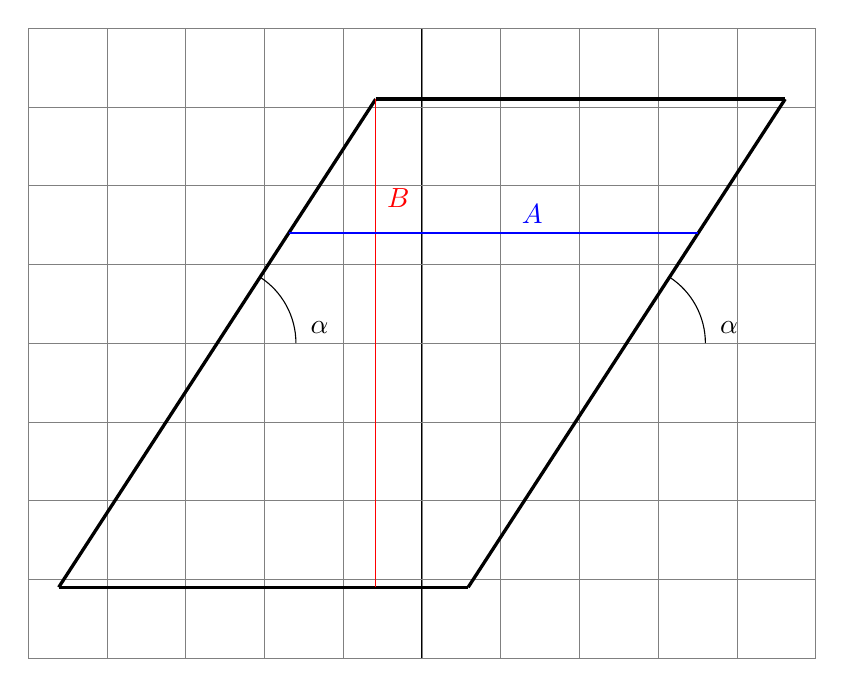
\begin{tikzpicture}
        \draw (-5,0) -- (5,0);
        \draw (0,-4) -- (0,4);
        \draw[step=1,gray,very thin] (-5,-4) grid (5,4);

        \draw[very thick] (-0.587,3.1) -- (4.613,3.1);
        \draw[very thick] (4.613,3.1) -- (0.587,-3.1);
        \draw[very thick] (0.587,-3.1) -- (-4.613,-3.1);
        \draw[very thick] (-4.613,-3.1) -- (-0.587,3.1);

        \draw[red] (-0.587,-3.1) -- (-0.587,3.1);
        \draw[blue] (-1.691,1.4) -- (3.509,1.4);

        \draw (-1.6,0) arc [start angle=0, end angle=57, radius=1];
        \draw (3.6,0) arc [start angle=0, end angle=57, radius=1];

        \draw (1.4, 1.4) node [color=blue,above] {$A$};
        \draw (-0.3, 1.6) node [color=red,above] {$B$};
        \draw (-1.3,0) node [above] {$\alpha$};
        \draw (3.9,0) node [above] {$\alpha$};
      \end{tikzpicture}

    \begin{ExampleIO}
    \egio{2.6\\3.1\\57}{35}
    \end{ExampleIO}
\end{task}
